\documentclass[sigconf]{acmart}
\usepackage{booktabs} % For formal tables

\hypersetup{bookmarksdepth=-2}

% Copyright
\setcopyright{rightsretained}

% DOI
\acmDOI{10.1145/3196369.3196392}

% ISBN
\acmISBN{978-1-4503-5717-3/18/05}

%Conference
\copyrightyear{2018}
\acmYear{2018}
\acmConference[ICGSE '18]{ICGSE '18: 13th IEEE/ACM International
Conference on Global Software Engineering }{May 27--29,
2018}{Gothenburg, Sweden}

\begin{document}
\title{Validation of Outsourcing Teams Work on Agile Projects\\
of Samsung R\&D Institute Brazil}
\subtitle{Extended Abstract}

\author{Gizelle S. Lemos}
\affiliation{%
  \institution{Samsung R\&D Institute Brazil}
  \city{Campinas}
  \state{SP}
  \country{Brazil}
}
\email{g.lemos@samsung.com}

\author{Marcia Cristina de C. Costa}
\affiliation{%
  \institution{Samsung R\&D Institute Brazil}
  \city{Campinas}
  \state{SP}
  \country{Brazil}
}
\email{m.costa@samsung.com}

\author{Tatiana D. Borghi}
\affiliation{%
  \institution{Samsung R\&D Institute Brazil}
  \city{Manaus}
  \state{AM}
  \country{Brazil}
}
\email{t.borghi@samsung.com}

\author{Paula G. Povoas}
\affiliation{%
  \institution{Samsung R\&D Institute Brazil}
  \city{Manaus}
  \state{AM}
  \country{Brazil}
}
\email{paula.povoas@samsung.com}

% The default list of authors is too long for headers.
\renewcommand{\shortauthors}{G. S. Lemos et al.}

\begin{abstract}
Samsung R\&D Institute Brazil (SRBR) is one of Samsung's research centers in the world in which there is research focused on software areas. SRBR teams have worked in collaboration with Samsung headquarter and outsourcing partners for producing software that aggregates value on Samsung products. SRBR has different partners with different levels of skill, maturity and that work in different contexts. For this reason, managing software development projects and guaranteeing the quality of resulting products have been challenging for SRBR. This experience report describes the process created to improve partners' management and proposes methods for tracking and improving the methods applied for validating the work delivered by outsourcing partners in order to guarantee that it meets Samsung quality requirements. 
\end{abstract}

\begin{CCSXML}
<ccs2012>
<concept>
<concept_id>10011007.10011074.10011099.10011105.10011109</concept_id>
<concept_desc>Software and its engineering~Acceptance testing</concept_desc>
<concept_significance>300</concept_significance>
</concept>
</ccs2012>
\end{CCSXML}

\ccsdesc[300]{Software and its engineering~Acceptance testing}


\keywords{Outsourcing management process, acceptance testing, outsourcing development}

\maketitle



\section{Introduction\label{sec:sec1}}

SRBR is one of the several research centers of Samsung. It is located in Brazil and geographically distributed in five different sites: three in southeast and two in the north of the country. 
Many research projects have been developed by SRBR demanded by Samsung Headquarter (HQ) in South Korea or by the local Latin America team. All software products produced by the SRBR teams must follows policies and processes defined by HQ and tailored to SRBR needs. Its teams develop software projects on different research areas such as artificial intelligence, machine learning, image\&video processing and security. Besides research projects, there are SRBR teams working on applications for local market and projects for contributing on platforms, such us Android \cite{Android18} and Tizen \cite{Tizen18}. 
 In both types of projects, not only the internal SRBR team has participated but also outsourcing partners, such us universities, research and development institutes and outsourced development organizations located in different regions of Brazil, Figure \ref{fig:mapa}.
 
\begin{figure}[!h]
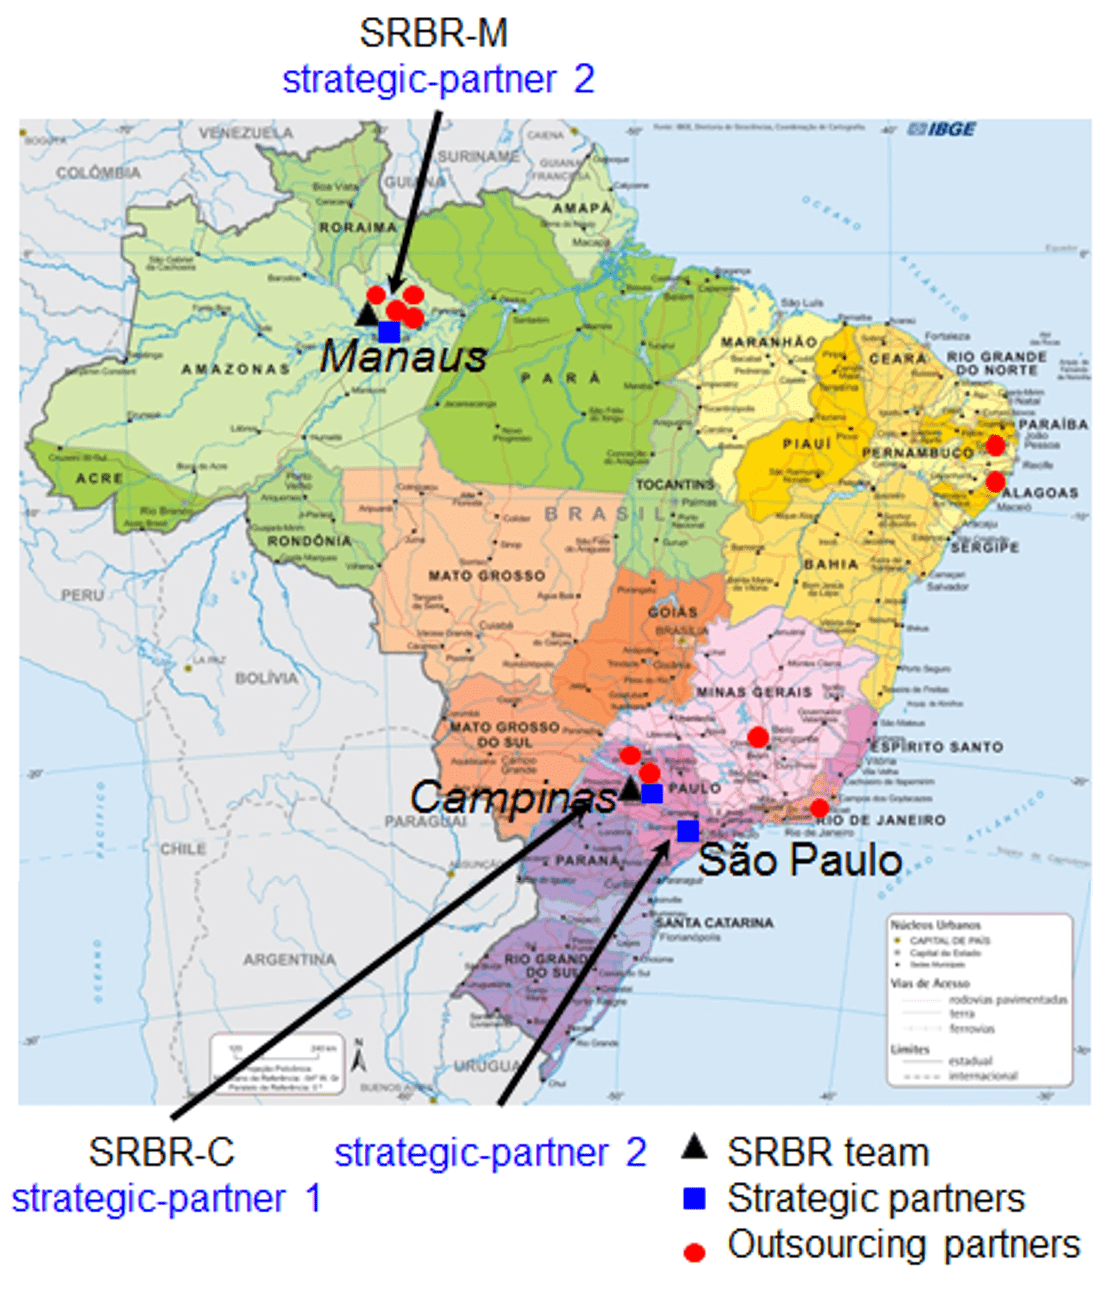
\includegraphics[height=2.2in, width=2.2in]{BrazilMap-min}
\caption{SRBR and Partner's Locations}
\label{fig:mapa}
\end{figure}

This business model that groups internal development teams and external partners on research projects has been heavily adopted by SRBR due to Brazilian incentive laws that concede tax exemptions to the company since it works with Brazilian research institutes and universities. 
Since 2015 SRBR has worked with about thirty partner companies. Difficulties present when working with outsourcing are related with the following aspects:
\begin{itemize}
\item Outsourcing companies have different levels of skill and maturity when considering software development process;
\item Different teams from the same outsourcing company have different levels of knowledge about SRBR SW Development Process; \cite{Costa18}
\item Teams from different types of outsourcing companies or companies from different country regions have different capabilities;
\item Outsourcing companies are located in different places, regions of Brazil.
\end{itemize}

In order to standardize the acceptance of work produced by SRBR' outsourcing partners, SRBR Software Engineering team (SRBR SE) defined on \textit{SRBR Technical Outsourcing Process} (Section \ref{sec:sec3}) some clear criteria for acceptance tests and on \textit{SRBR Software Development Process} a set of activities applicable during acceptance that have been applied on the majority of ongoing projects with participation of outsourcing partners.

Whenever a \textit{release} is delivered by a partner, SRBR team performs acceptance activities which results on a verdict about the \textit{release}' quality. All releases should be formally accepted by SRBR before being incorporated into the product.

The purpose of this report is to present the experience of SRBR, in special of SRBR SE team in working with outsourcing partners and how SRBR are accepting the deliverables. We will present some results of projects developed in 2017 and projects in developing in 2018.

On next section we describe \textit{SRBR Software Development Process} and the processes that support the outsourcing activities (Section \ref{sec:sec2}). On Section \ref{sec:sec3} we detail how SRBR  have accepted deliverables from outsourcing organizations, some results obtained and what we need to improve. On section 4 we present the conclusions of our experience.

\section{SRBR Software Development Process \label{sec:sec2}}

SRBR software projects have been developed following a SRBR SW Development Process. The SRBR SW Development Process was tailored from Samsung Engineering Process (SEP) defined by HQ and references ISO/IEC 12207 \cite{IEEE12207-08}, Figure \ref{fig:devprocess}.

\begin{figure}[!h]
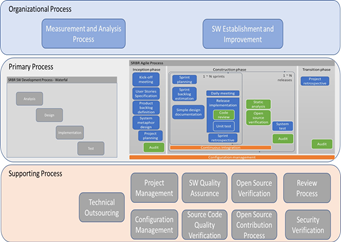
\includegraphics[height=2in, width=3in]{DevProcess}
\caption{SRBR SW Development Process Overview}
\label{fig:devprocess}
\end{figure}

Sections \ref{sec:sec2-1} and \ref{sec:sec2-2} describe the processes used during validation of outsourcing teams. An overview of entire SRBR SW Development Process is available on \cite{Costa18}.

\subsection{SRBR Technical Outsourcing Process \label{sec:sec2-1}}

The SRBR Technical Outsourcing Process comprises four major phases:

\begin{itemize}
\item \textit{Plan outsourcing project}: define the scope and strategy for outsourcing;
\item \textit{Prepare outsourcing project}: prepare Request for Proposal (RFP), selected outsourcing organization, negotiate and sign off contract and statement of work;
\item \textit{Track outsourcing project}: monitor the progress of development of the project, verify and validate deliverables according statement of work, conduct acceptance tests;
\item \textit{Close outsourcing project}: project transfer (transfer the technology developed by outsourcing organization to SRBR internal development team when it is applicable), conduct lessons learned meeting, evaluate outsourcing organization and close contract.
\end{itemize}

\subsection{SRBR Agile Process \label{sec:sec2-2}}

\textit{SRBR SW Development Process} was defined and established considering mandatory and non-mandatory phases, activities and deliverables that software development projects follow. It describes either Waterfall life-cycle and Agile methodology as reference. From Agile methodologies, \textit{SRBR SW Development Process} considers:

\begin{itemize}
\item From Xtreme programming \cite{XP13}: User stories, system metaphor, simple design, release planning, continuous integration;
\item From Scrum \cite{Scrum18}: Sprints, estimation, daily meetings, retrospective meetings, burn-down/burn-up charts;
\item From Lean software development \cite{Poppendieck:2003:LSD}: Kanban board.
\end{itemize}

Besides activities from Agile methodologies, \textit{SRBR SW Development Process} defines a set of activities for software quality assurance:

\begin{itemize}
\item \textit{Static analysis}: automated detection of potential errors through static code analysis without running the target program. Defects on code and build without preparation of test cases or program execution. It supports a wide range of languages and checkers for versatility to deal with functions needed;
\item \textit{Open source verification}: source code analysis to verify if open source components included into the software project are allowed considering rules for commercial software;
\item \textit{System test}: test performed by an independent team that may include conformance, stress, integration, and usability tests of software product releases;
\item \textit{Code review}: technical evaluation by developers contributing for improvement and fixing of source code before integrating it on a product. 
\item \textit{SW quality assurance audits}: periodical SW audits performed to verify the adherence of projects with respect to their pre-specified SW Development Process;
\item \textit{Configuration management}: identification of configuration items (CI) and baselines definition, control  changes in project's CIs assuring the integrity of the software produced.

\end{itemize}

Quality assurance activities are mandatory to SW projects and most of them have specific criteria that projects must achieve before development is finished.

Agile concepts and quality assurance activities have been applied on phases of the software development life cycle on mentioned below and summarized on Figure \ref{fig:agile}:

\begin{itemize}
\item \textit{Inception phase}: beginning of project in which occurs definition of plans, initial backlog and initial idea about Software architecture;
\item \textit{Construction phase}: execution of N sprints in order to generate releases according prioritization defined by client (product owner);
\item \textit{Transition phase}: technology transference, lessons learned and completion of project.
\end{itemize}

\begin{figure}[!h]
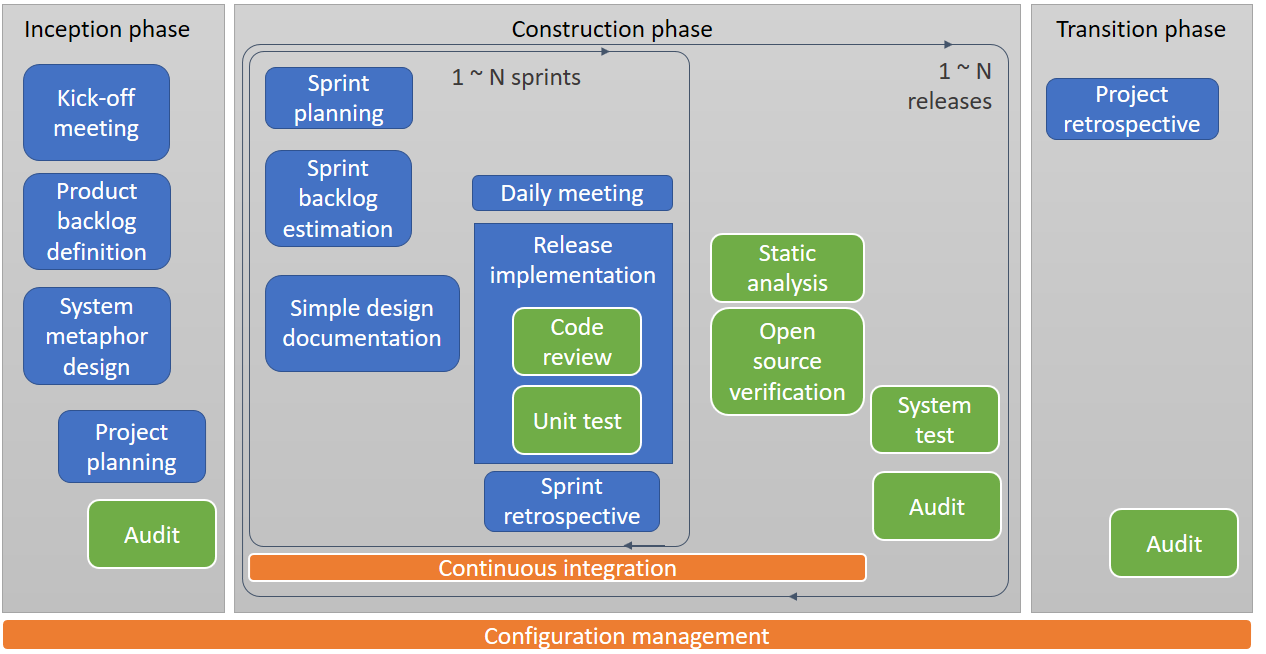
\includegraphics[height=2in, width=3in]{SRBRAgile}
\caption{Phases of Agile methodology defined in SRBR SW Development Process}
\label{fig:agile}
\end{figure}

\textbf{Inception Phase}

The focus of this phase is plan main project milestones and document the first version of the project's planning deliverables. All team members participate on a kick-off meeting and define the tailoring needs for the project considering the \textit{SRBR SW Development Process}. 

Project team documents initial product backlog and system metaphor (high level software architecture) to be able to plan the projects' releases schedule. 

After definition of project plans, an audit is performed by SRBR SE team in order to verify if all required activities and deliverables have been generated. The summary of activities and deliverables of Inception Phase is on Table \ref{tab:inception}:

\begin{table}[h]
  \caption{Summary of Inception Phase}
  \label{tab:inception}
  \begin{tabular}{p{2.5cm}p{5.5cm}}
    \toprule
    Activities&Mandatory Deliverables\\
    \midrule
    Kickoff Meeting & Kickoff Meeting	Kick-off Meeting notes, Project Tailoring Document\\
    User Stories Specification & Initial Product Backlog\\
    System Metaphor Definition & System Metaphor\\
    Project Planning & Agile Release Plan, SW Configuration Management Plan, SW Quality Assurance Plan\\
    Audit & Inception Phase Audit Report\\
  \bottomrule
\end{tabular}
\end{table}

\textbf{Construction Phase}

During this phase, the product is developed and released according with project strategy and planning defined in inception phase. One release can be comprise by one or more sprints. During the sprints, project team performs for each sprint: sprint' planning, backlog estimation, Daily meetings, software source code generation, unit tests, Code review, and sprint retrospective.

Whenever, after the end of sprint, a release has been planned, project team performs some activities in order to guarantee its quality: static analysis, open source verification, system test and release demonstration (to product owner).

Automatic builds, unit tests and static analysis run in the continuous integration system increasing the time available for issues resolution.

Before the delivery of each release, SRBR SE team performs an audit in order to verify if all software quality assurance activities were performed and criteria achieved. The summary of activities and deliverables of Construction Phase is on Tables \ref{tab:construction-sprint} and \ref{tab:construction-release}.

\begin{table}[h]
  \caption{Summary of Construction Phase - Sprint activities }
  \label{tab:construction-sprint}
  \begin{tabular}{p{2.5cm}p{5.5cm}}
    \toprule
    Activities&Mandatory Deliverables\\
    \midrule
    Sprint Planning & Sprint planning report (sprint goal, sprint backlog, product backlog, sprint needs), sprint backlog estimation\\
    Open source verification & Open Source Pre-review Report\\
    Daily Meeting & Burndown/Burnup charts updated\\
    Source Code Implementation & Source code reviewed on repository, Unit Tests Reports \\
    Sprint Retrospective & Sprint Retrospective Report\\
  \bottomrule
\end{tabular}
\end{table}

\begin{table}[h]
  \caption{Summary of Construction Phase - Release activities}
  \label{tab:construction-release}
  \begin{tabular}{p{3.5cm}p{4.5cm}}
    \toprule
    Activities&Mandatory Deliverables\\
    \midrule
    Static Analysis & SW Code Quality Verification Report\\
    Open source verification & Open Source Verification Report\\
    System Test & System Test Plan, System Test Cases, System Test Report\\
    Audit & Construction Phase Audit Report\\
  \bottomrule
\end{tabular}
\end{table}

\textbf{Transition Phase}

The last phase of \textit{SRBR SW Development Process} focus on project closure. All team members participate on the lessons learned meeting and the final report of the project is documented by project leader comparing planning and achievements for the project. Final product release is delivered and audit verifies all product deliverables. Below  table (Table \ref{tab:transition}) lists activities and mandatory deliverables of this phase.

\begin{table}[h]
  \caption{Summary of Transition Phase}
  \label{tab:transition}
  \begin{tabular}{p{2.5cm}p{5.5cm}}
    \toprule
    Activities&Mandatory Deliverables\\
    \midrule
    Project retrospective & Lessons Learned Meeting Notes\\
    Project completion & Project Completion Report\\
    Audit & Transition Phase Audit Report\\
  \bottomrule
\end{tabular}
\end{table}

\section{Acceptance Activities\label{sec:sec3}}

Due to problems presented in Section \ref{sec:sec1} regarding outsourcing management and result's evaluation, SRBR SE Team, responsible for defining and improving \textit{SRBR SW Development Process} and for supporting development teams on process deployment in projects, decided to define complimentary activities and make some improvements on SRBR Technical Outsourcing Process for projects that involve development teams from outsourcing partners. The improved process has been applied in projects since 2017.

Below are presented changes on SRBR Technical Outsourcing Process and on SRBR Software Development Process.

The first activity included on projects is \textit{Review and Detail of Statement of Work}. In summary, this document describes the work scope, project deliverables, schedule of releases and acceptance criteria for the partners' work. However, there before process improvement there were no template or minimum mandatory set of information for it. 

SRBR SE team defined a document named SW Annex that summarizes all activities and deliverables expected by software development phase. Nowadays, it is part of Request of Proposal (RFP) sent to outsourcing candidates before partner's choice. 

When an outsourcing is selected, SW Annex is included in Statement of Work and/or in Partnership' Agreement. SW Annex details:

\begin{itemize}
\item The type of outsourcing project, based on the scope of development: e.g.  requirements to system test, design to system test, implementation to system test, requirements to implementation;
\item Mandatory activities;
\item Mandatory deliverables and minimum content;
\item Roles and responsibilities during development;
\item Releases acceptance criteria. Specific acceptance criteria have been defined for some activities performed during the project. The focus is on construction phase - release activities:
  \begin{itemize}
  \item Static analysis: 
      \begin{itemize}
      \item All potential defects should be classified as defect or false-positive;
      \item All potential defects classified as false-positives must be justified and audited;
      \item All defects of critical severity must be fixed;
      \item A maximum of one defect may be left open in one million lines of code;
      \end{itemize}
  \item Open source verification: only allowed open source components must be adopted by partners' development teams and their licenses obligations must be abide;
  \item System test: performed and reported by outsourcing team before each release delivery: 
      \begin{itemize}
      \item All defects found by partner's test team must be classified according severity: A, B, C in witch A is more severe and C is less severe;
      \item Al defects with severities A and B must be resolved before release delivery to SRBR;
      \end{itemize}
   \item Acceptance test: on test performed by SRBR after all releases delivery by partner are expected no defects of severity A and B.
   \end{itemize}
\end{itemize}

Based on the Statement of Work, SRBR SE team performs quality assurance activities as defined on SW Quality Assurance Plan and acceptance test activities for each release. In parallel, SRBR project team defines
what portion of the product backlog will be under partner's responsibility. The outsourcing scope is the target for validation from the point of view of the product owner and of SW Annex criteria. In case of projects with participation of outsourcing partners, a member of SRBR team represents the product owner on release acceptance. 

The Construction Phase starts after the agreement between SRBR and partner about plans defined on Inception Phase. On SRBR software process each release is a result of one or more sprints produced according to scope and schedule of Statement of Work. 

For each release delivered by outsourcing team, SRBR performs the set of activities for quality assurance: static analysis, open source verification and acceptance test. Only if the release meets all acceptance criteria it is considered \textit{Accepted} by SRBR. In addition, all deliverables that compose the release are verified during the Construction Phase Audit. 

Below are presented some results of eleven closed and ongoing projects in the period of 2017/2018 that have followed this improved process.

\textbf{Static Analysis}

In projects in which static analysis is applicable (only C, C++, C\# and Java source code), SRBR tool (proprietary tool developed by HQ) identified more than 350 Critical and Major issues that escaped in code review (Figure \ref{fig:static-analysis}).

\begin{figure}[!h]
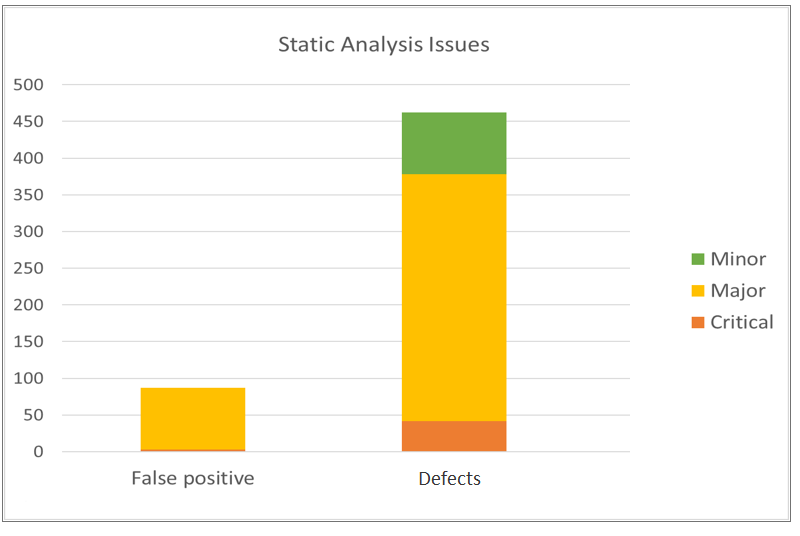
\includegraphics[height=1.3in, width=2.8in]{StaticAnalysis}
\caption{Static Analysis results}
\label{fig:static-analysis}
\end{figure}

\textbf{Open Source Verification}

During verification of open source components incorporated by partner's team we have used BlackDuck Protex\texttrademark tool\cite{Protex}, we identified the usage of 23 open source components and we could guarantee that those projects are compliant with Samsung's open source policies (Figure \ref{fig:opensource}).

\begin{figure}[!h]
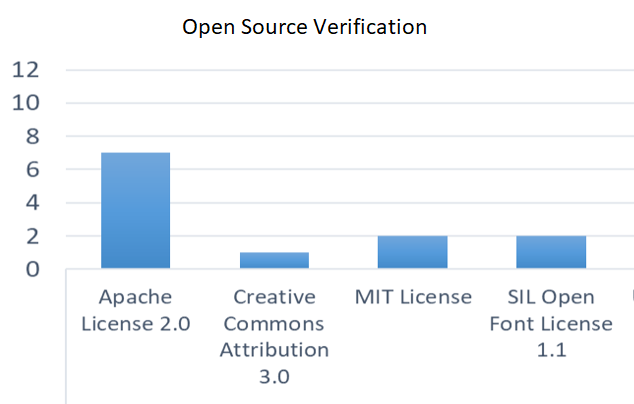
\includegraphics[height=1.5in, width=2.8in]{OpenSource}
\caption{Open source verification results}
\label{fig:opensource}
\end{figure}

\textbf{System Tests}

SRBR SE team verified all system test reports delivered by outsourcing teams. System Test Reports are compared with SRBR Acceptance Test Reports in order to verify what defects escaped during partner's tests. 

\textbf{Acceptance Tests}

SRBR SE team performs acceptance test activity after all releases delivery. For verified releases were identified defects of severity A and B that escaped during system test cycles (around 38\% of defects found). In this case the release delivered was rejected by SRBR and new version was generated after defects fixing by partners. 

During the acceptance tests, SRBR SE realized that was difficult to classify the severity of some defects found based on actual severity definitions when testing some types of projects, e.g. games.

Figure \ref{fig:accept-testing} illustrates defects found during acceptance test divided by defect category and project type.

\begin{figure}[!h]
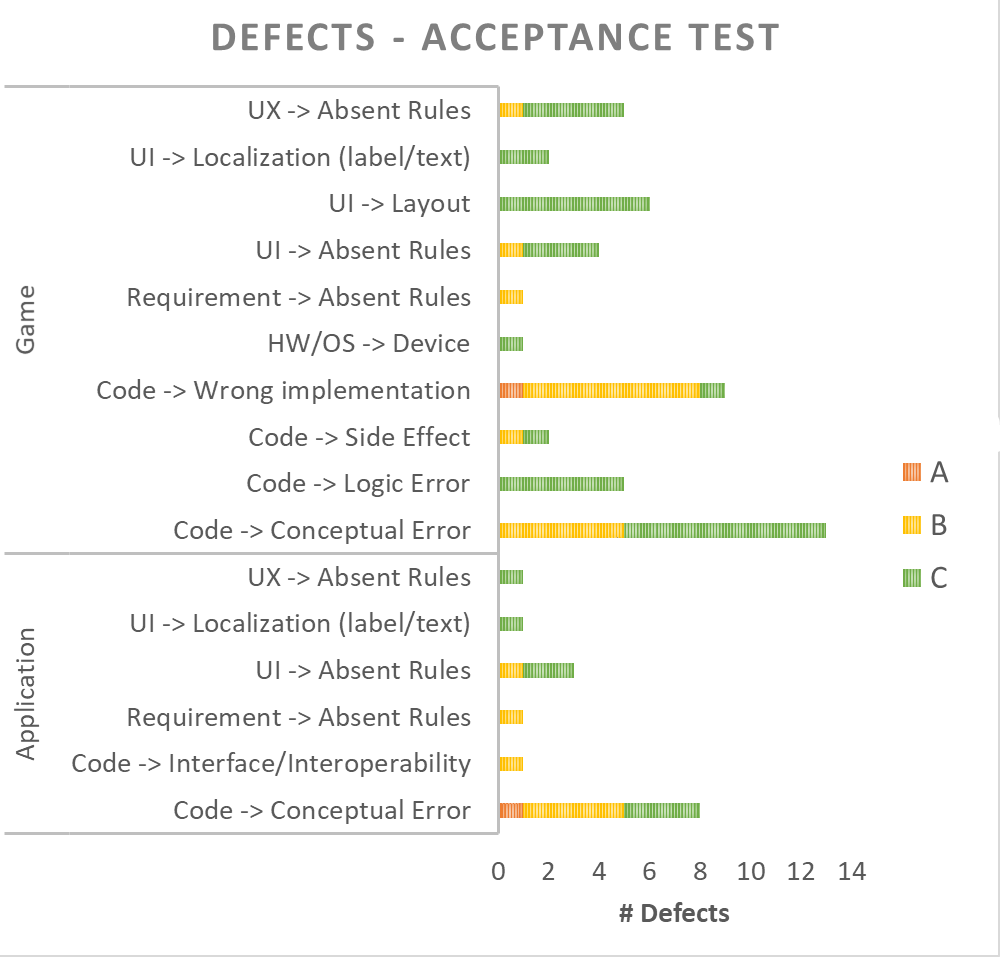
\includegraphics[height=2.5in, width=2.8in]{AcceptanceTest}
\caption{Acceptance Test defects by category}
\label{fig:accept-testing}
\end{figure}

\textbf{Audits}

On audits performed by SRBR SE team a set of issues was found. All issues were classified as non-conformities or improvement opportunities. Most of issues identified on outsourcing teams are related with configuration management and project management processes (Figure \ref{fig:audit}). It demonstrate that SRBR and partners should work to improve the level of maturity of these organizations in these process areas.

\begin{figure}[!h]
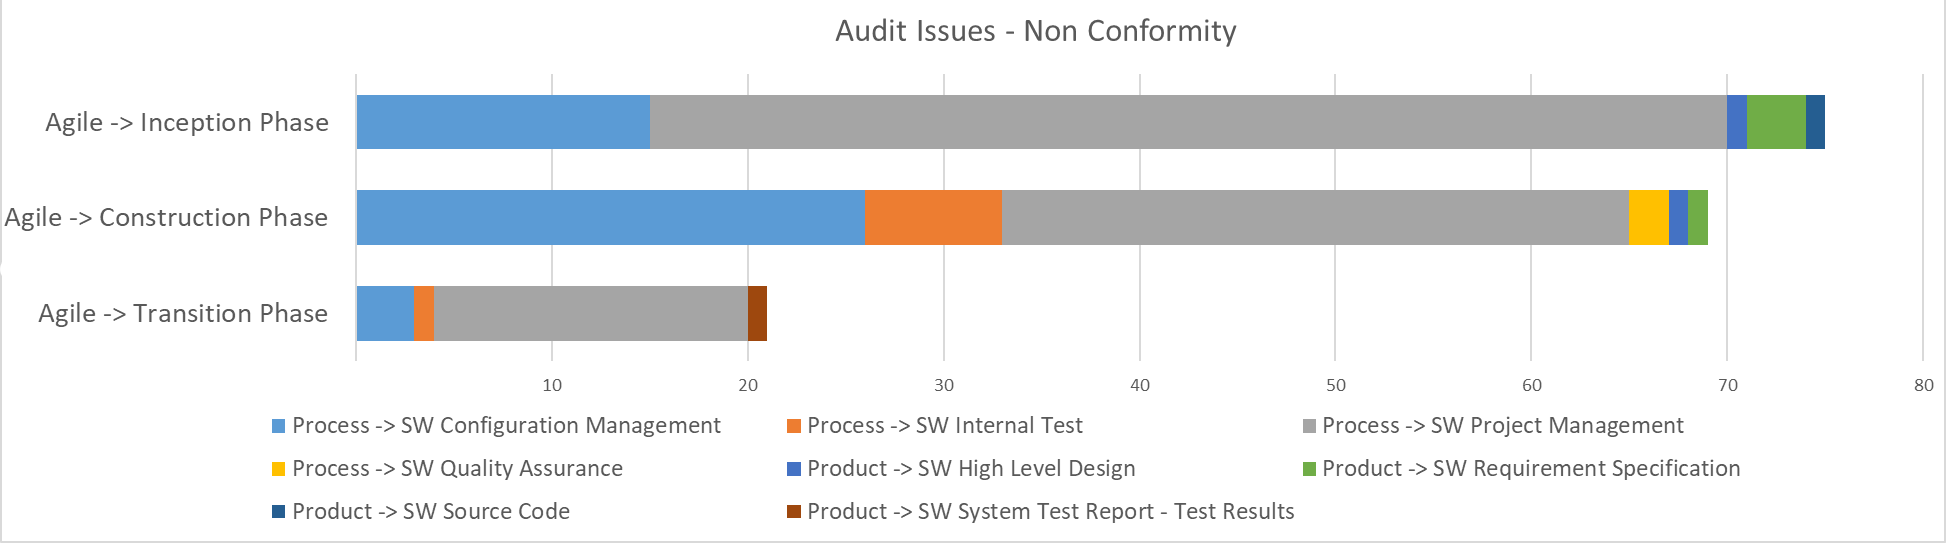
\includegraphics[height=1.5in, width=3in]{Audit}
\caption{Audit Issues}
\label{fig:audit}
\end{figure}

\section{Conclusions}
SRBR has obtained some gains performing the formal acceptance of the outsourcing work: 
\begin{itemize}
\item Independently of partner's company or SRBR team that manages the software project under development the criteria for releases acceptance are the same;
\item Acceptance test has avoided that product releases with escaped defects (not found by partner's test teams) were delivered to SRBR; 
\item Open source verification has guaranteed that only allowed open source components have been adopted by partners' teams and also their licenses obligations were abide; 
\item Audits have helped on standardize deliverables produced by partners facilitating the understanding and analysis of by SRBR teams;
\item Audits also have helped teams to find weakness points on agile practices understanding and execution by partners;
\item Different improvement opportunities were identified such as:
	\begin{itemize}
	\item Possibility of Use the results of each project to evaluate and select outsourcing companies;
	\item Feedback about the quality of process and deliverables was uses to establish an action plan to improve the capability of outsourcing organizations;
	\item Definition of severity of defects has been reviewed and specialized by project type, such us games and applications in order to facilitate classification of defects.
    \end{itemize}
\end{itemize}

\bibliographystyle{ACM-Reference-Format}
\bibliography{ICGSE_bib_file}

\end{document}
